\documentclass[a4paper,12pt]{article}

%% Language and font encodings
\usepackage[english, russian]{babel}
\usepackage[utf8x]{inputenc}
\usepackage{blindtext}
\usepackage[T1]{fontenc}
\usepackage[T2A]{fontenc}
\usepackage[a4paper,top=1.5 cm,bottom=2cm,left=3cm,right=3cm,marginparwidth=1.75cm]{geometry}
%% Useful packages
\usepackage{amsmath, amssymb}
\usepackage{wrapfig}
\usepackage{graphicx}
\usepackage[usenames]{color}
\usepackage[T1]{fontenc}
\usepackage{tikz}
\usetikzlibrary{arrows}
\usetikzlibrary{decorations.pathreplacing}
\usepackage[T2A]{fontenc}
\usepackage{color}
\usepackage{circuitikz} 
\usetikzlibrary{circuits}
\usetikzlibrary{circuits.ee}
\usetikzlibrary{circuits.ee.IEC}
\usetikzlibrary{circuits.logic.IEC}
\graphicspath{{pic/}}
\definecolor{water} {rgb} {0.667, 0.855, 1}
\usepackage{pgfplots}
\usepackage{pgfplotstable}

\title{МОДЕЛИРОВАНИЕ ОПТИЧЕСКИХ ПРИБОРОВ И ОПРЕДЕЛЕНИЕ ИХ УВЕЛИЧЕНИЯ}
\date{Работа 4.1.2}
\author{Ляликова Ирина, Б05-911}
\begin{document}
	
	\vspace{0.5 cm}
	\maketitle
	\vspace{0.5 cm}
	
	\textbf{Цель работы:} Определить фокусные расстояния собирающих и рассеивающих линз, смоделировать ход лучей в трубе Галилея, трубе Кеплера и микроскопе, определить их увеличение. \\
	
	\textbf{В работе используются:} оптическая скамья, набор линз, экран, осветитель со шкалой, зрительная труба, диафрагма, линейка.\\
	
	\textbf{Экспериментальная установка.} Набор линз, осветитель, экран, зрительная труба, необходимые для моделирования оптических приборов, устанавливаются при помощи рейтеров на оптической скамье. Предметом служит
	миллиметровая шкала или сетка, нанесённая на матовое стекло осветителя.
	
	\textbf{Центрирование линз.} При юстировке любых оптических приборов важно правильно центрировать входящие в систему линзы. Проходя через плохо
	отцентрированную систему линз, лучи света отклоняются в сторону и могут
	вообще не доходить до глаза наблюдателя. Центрировать линзы следует как
	по высоте, так и в поперечном направлении (для чего линзы крепятся на, поперечных салазках). Подробно с правилами центрировки Вы познакомитесь
	при выполнении задания.
	
	\textbf{Юстировка коллиматора.} При составлении моделей телескопических
	систем необходимо иметь удалённый объект. В качестве такого объекта обычно используется бесконечно удалённое изображение предмета (шкалы осветителя), установленного в фокальной плоскости положительной линзы. Лучи,
	выходящие из одной точки предмета, пройдя через линзу, образуют параллельный пучок. Устройство такого рода называется \textit{коллиматором}.

	Для юстировки коллиматора удобно использовать вспомогательную зрительную трубу, предварительно настроенную на бесконечность. Передвигая
	линзу коллиматора вдоль скамьи, добиваются появления резкого изображения предмета в окуляре зрительной трубы.
	
	\textbf{Измерение фокусных расстояний линз.} Для того, чтобы сознательно
	моделировать оптические инструменты, нужно знать фокусные расстояния
	линз, которые могут быть использованы в качестве объектива или окуляра модели. Фокусные расстояния тонких положительных линз проще всего
	найти с помощью вспомогательной зрительной трубы, установленной на, бесконечность. Работа выполняется так же, как при юстировке коллиматора.
	
	При определении фокусного расстояния отрицательной линзы предметом
	служит изображение шкалы, которое даёт вспомогательная положительная
	линза.
	
	\section*{Ход работы}
	
	\subsection*{Центрировка элементов оптической системы}
	\begin{enumerate}
		
		\item В имеющемся наборе присутствуют собирающие линзы с приближёнными значениями фокусных расстояний (определены с помощью фокусировки удалённого источника на листе бумаги):
		\begin{center}
			\begin{tabular}{|c|c|c|c|c|}
				\hline
				№ линзы & 1 & 2 & 3 & 4 \\ \hline
				$f$, см & $8,5\pm1$ & $10\pm1$ & $20\pm1$ & $40\pm1$ \\ \hline
			\end{tabular}
		\end{center}
		Также в наборе есть одна рассеивающая линза, фокусное расстояние которой будет определено в следующих пунктах.
		
		\item Собрали и отцентрировали все положительные линзы, добавляя их последовательно к системе (не убирая уже отцентрированные). Для центрировки рассеивающих линз пользовались уже отцентрированной положительной линзой, расположив её впереди отрицательной.
		
	\end{enumerate}

	\subsection*{Определение фокусных расстояний тонких линз с помощью зрительной трубы}
	\begin{enumerate}
		\item Для определения фокусных расстояний линз с помощью зрительной трубы настроили трубу на бесконечность.
		
		\item Установили собирающую линзу на расстоянии от предмета примерно равном фокусному (рис. 1). На небольшом расстоянии от линзы закрепили трубу, настроенную на бесконечность.
							
		\begin{figure}
			\begin{center}
				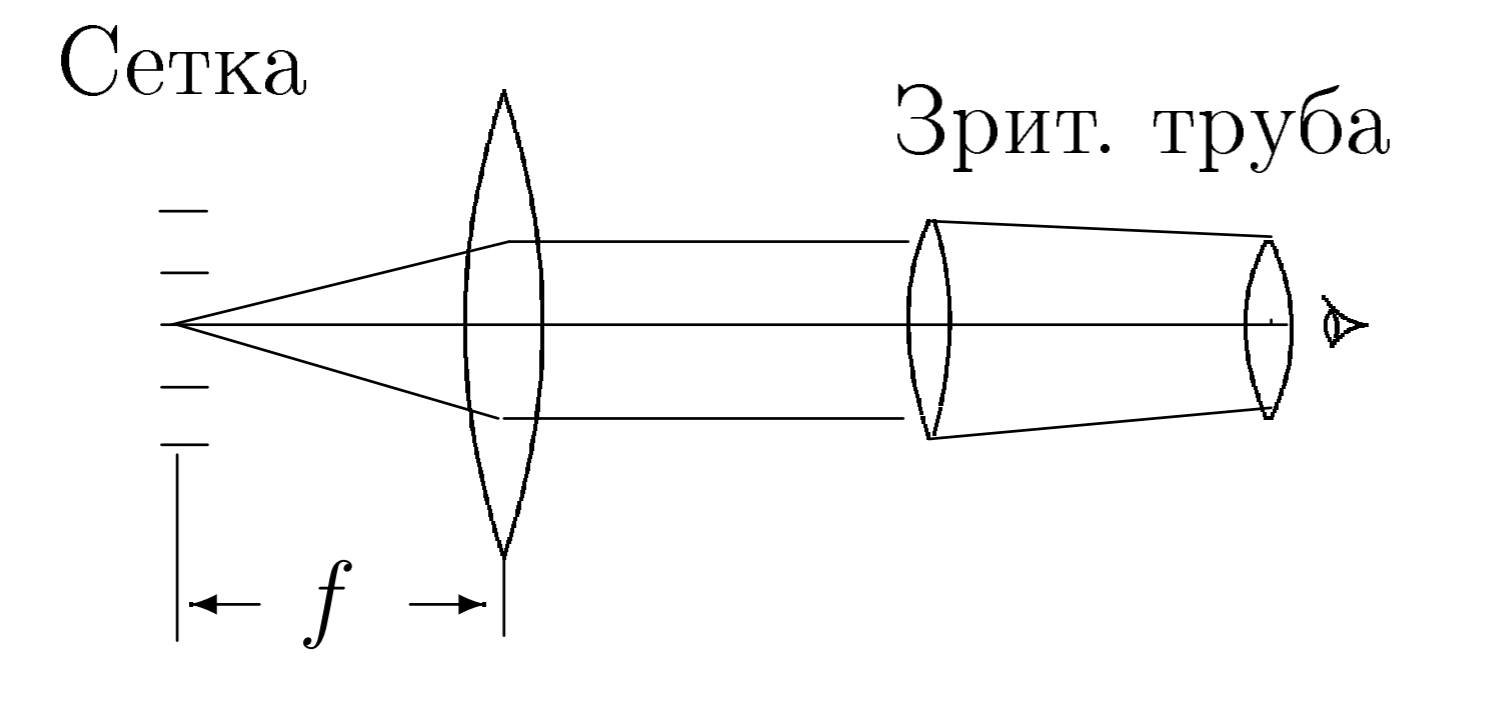
\includegraphics[width = 0.5\textwidth]{412-1.png}
				\caption{Определение фокусного расстояния собирающей линзы}
			\end{center}
		\end{figure}
			
		Диафрагма диаметром $a=1$ см, надетая на ближнюю к осветителю линзу, делает пучок параксиальным (близким к оси), при этом растёт чёткость изображения за счёт уменьшения сферической аберрации.
		
		Передвигая линзу вдоль скамьи, получили в окуляре зрительной трубы
		изображение предмета --- миллиметровой сетки. При этом расстояние между
		предметом и серединой тонкой линзы (между проточками на оправах) равно фокусному.
		
		\item Повернув линзу другой стороной к источнику, повторили измерения фокусного расстояния, чтобы по результатам измерений сделать вывод, можно ли считать линзу тонкой.
		
		\item  Измерили фокусные расстояния всех положительных линз при помощи зрительной трубы:
		
		\begin{center}
			\begin{tabular}{|c|c|c|c|c|}
				\hline
				№ линзы & 1 & 2 & 3 & 4 \\ \hline
				$f_1$, мм & 8,5 & 10,0 & 19,5 & 32,5 \\ \hline
				$f_2$, мм & 8,7 & 10,0 & 19,5 & 32,0 \\ \hline
			\end{tabular}
		\end{center}
	
		Здесь расстояния определены с погрешностью 2~мм. Значения, полученные 
		
		\item Для определения фокусного расстояния тонкой рассеивающей линзы сначала получили на экране увеличенное изображение сетки при помощи одной короткофокусной собирающей линзы. Измерили расстояние между линзой и экраном $a_0 = 49{,}0$ см.
									
		\begin{figure}
			\begin{center}
				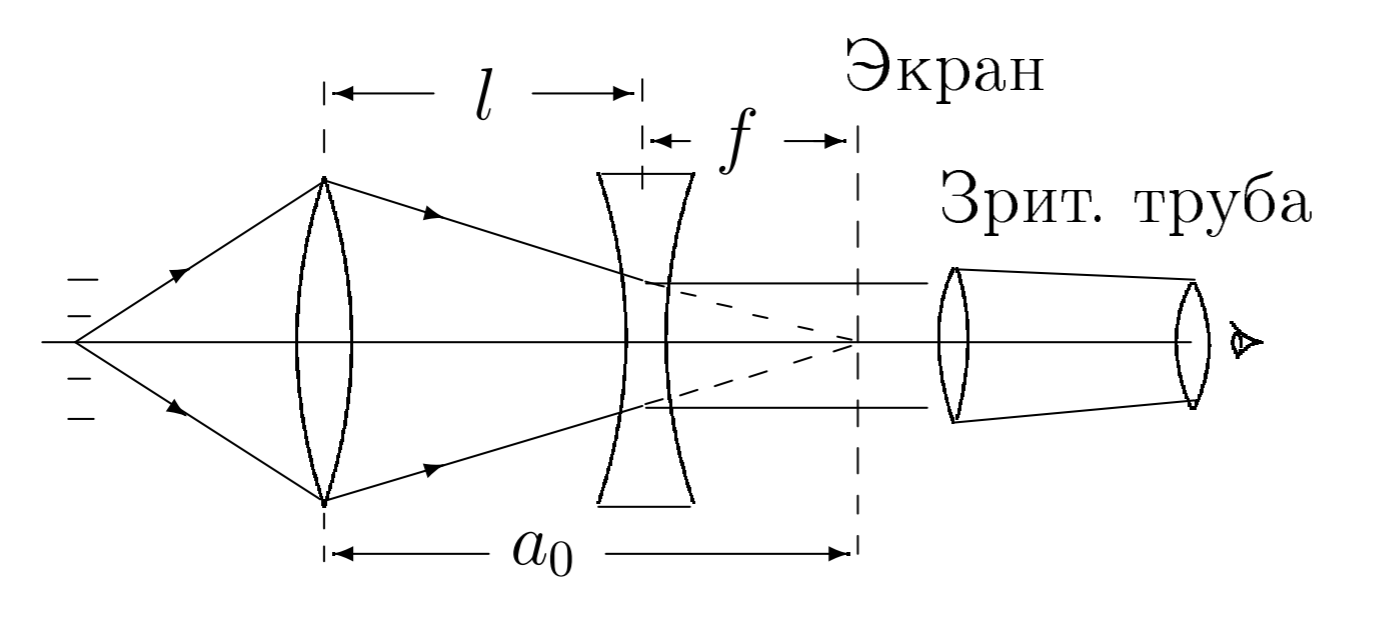
\includegraphics[width = 0.5\textwidth]{412-2.png}
				\caption{Определение фокусного расстояния рассеивающей линзы}
			\end{center}
		\end{figure}
	
		\item Разместили сразу за экраном трубу, настроенную на бесконечность, и закрепили её. Убрали экран и поставили на его место исследуемую рассеивающую линзу (рис. 2). Отцентрировали световой пучок с помощью листа бумаги. Перемещая рассеивающую линзу, нашли в окуляре зрительной трубы резкое изображение сетки. Измерив расстояние между линзами $l = 40{,}0$ см, рассчитаем фокусное расстояние рассеивающей линзы:
		\begin{equation*}
		|f_5| = l - a_0 = 9{,}0\pm0{,}2\text{ см}.
		\end{equation*}
		
		\item Повторили измерения, повернув рассеивающую линзу другой стороной к источнику и получили те же результаты.
	\end{enumerate}
	\subsection*{Телескоп Кеплера}
	\begin{enumerate}
		\item Из имеющегося набора взяли две собирающих линзы для создания модели
		зрительной трубы Кеплера с увеличением 2-3 (рис. 3). В качестве коллиматора использовали линзу с фокусным расстоянием $f = 19{,}5$ см (при этих
		условиях размер изображения предмета не превышает размера поля
		зрения вспомогательной зрительной трубы).
											
		\begin{figure}
			\begin{center}
				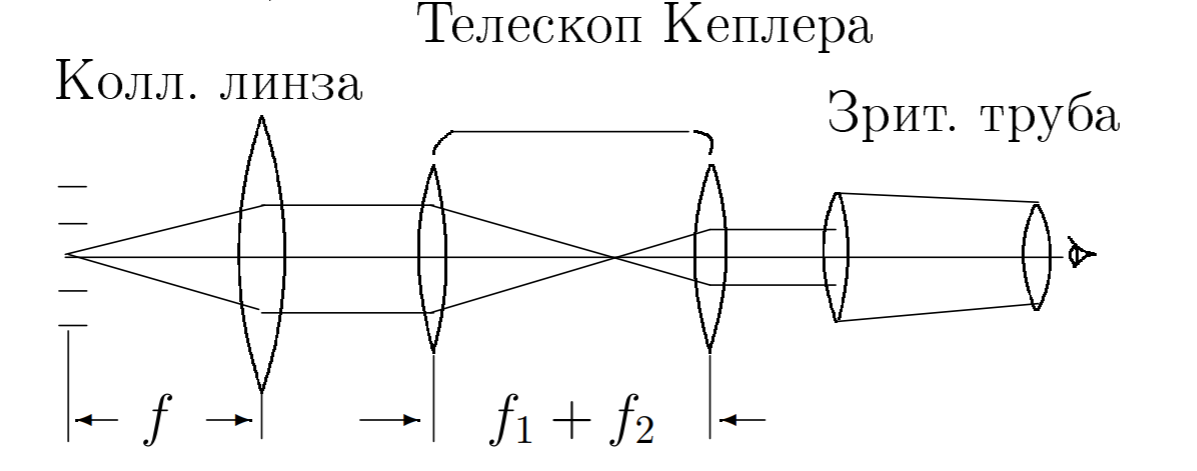
\includegraphics[width = 0.5\textwidth]{412-3.png}
				\caption{Модель телескопа}
			\end{center}
		\end{figure}
		
		\item Для последующих расчётов увеличения определили размер изображения $h_1 = 31/4 =7{,}75\pm0{,}25$ делений одного миллиметра шкалы осветителя. Очевидно, $h_1 = k\alpha_1$, где $k$ --- некоторый коэффициент, характеризующий увеличение зрительной трубы, $\alpha_1$ --- угловой размер изображения миллиметрового деления шкалы осветителя, наблюдаемого через коллиматор.
		
		\item Собрали модель телескопа: линзу с максимальным фокусным расстоянием --- объектив модели --- расположили почти вплотную к линзе коллиматора, окуляр --- на расстоянии, примерно равном сумме фокусных расстояний обеих линз телескопа.
		Закрепили вспомогательную зрительную трубу за окуляром модели и отцентрировали световое пятно при помощи листа бумаги. Слегка перемещая окуляр модели вдоль оптической скамьи, получили изображение миллиметровой сетки в окуляре вспомогательной трубы.
		
		Измерили расстояние между объективом и окуляром телескопа 
		\begin{equation*}
		s = 42{,}5\pm0{,}2\text{ см}
		\end{equation*}
		и сравнили его с суммой фокусных расстояний:
		\begin{equation*}
			f_1+f_2 = 32{,}0\text{ см} + 10{,}0\text{ см} = 42{,}0\pm0{,}4\text{ см}.
		\end{equation*}
		
		Значения сходятся с хорошей точностью.
		
		\item Рассчитали увеличение исследуемой модели телескопа через отношение фокусных расстояний:
		\begin{equation*}
		N_T = \dfrac{\alpha'}{\alpha} = -\dfrac{f_1}{f_2} = -3{,}20\pm0{,}09.
		\end{equation*}
		
		\item Для определения увеличения телескопа через отношение углов, под кото-
		рыми объект виден через телескоп и без него, определили размер $h_2$ изоб-
		ражения миллиметрового деления шкалы осветителя в делениях окулярной
		шкалы вспомогательной трубы: $h_2 = k\alpha_2$. Здесь $\alpha_2$ --- угловой размер изображения миллиметрового деления шкалы при наблюдении через исследуемый телескоп.
		
		\begin{equation*}
		h_2 = 25\pm1\text{ дел./мм}.
		\end{equation*}
		
		Сравнив $h_2$ с величиной $h_1$, полученной в п. 2 без телескопа, определили
		увеличение телескопа, используя формулу
		\begin{equation*}
		N_T = -\dfrac{h_2}{h_1} = -3{,}2\pm0{,}3.
		\end{equation*}
		 \item Определили увеличение телескопа, измерив диаметр оправы его объектива $D_1 = 34\pm1$~мм и диаметр изображения этой оправы в окуляре $D_2=11\pm1$~мм. Для этого отодвинули вспомогательную трубу и расположили экран за окуляром телескопа. Сняли диафрагму с коллиматора и убедились, что световое пятно полностью освещает объектив телескопа и проходит через окуляр. Отодвигая экран от окуляра, получили на нём чёткое изображение оправы объектива. Поднеся к объективу какой-нибудь предмет (например, край линейки), убедились, что наблюдается именно изображение оправы объектива. Измерили диаметр объектива и диаметр его изображения. Рассчитали увеличение трубы через диаметры:
		 
		 \begin{equation*}
		 N_T = -\dfrac{D_1}{D_2} = -3{,}1\pm 0{,}4.
		 \end{equation*}
		 
		 \item Результаты измерения увеличения телескопа разными методами совпали с точностью до погрешности.
	\end{enumerate}
	\subsection*{Труба Галилея}
	\begin{enumerate}
	\item Переход от трубы Кеплера к трубе Галилея осуществили, не изменяя положения коллиматора и объектива, при этом вместо собирающей окулярной линзы телескопа поставили рассеивающую линзу $f_5$ на расстоянии от объектива, равном разности фокусов объектива и окуляра. Дальнейшие измерения выполнялись в том же порядке, что и в случае астрономической трубы.
	
	\item Получили $l = 25{,}0\pm0{,}2$ см, при значении $f_1 + f_5 = 25{,}0\pm0{,}4$ см. 
	
	Увеличение разными методами:
	\begin{equation*}
		h_2 = 31\pm1\text{ дел./мм},\;\;\;\; h_1 = \dfrac{31}{4}\text{ дел./мм},
	\end{equation*}
	откуда
	\begin{equation*}
	N_G = 4{,}0\pm0{,}2.
	\end{equation*}
	Через фокусные расстояния получили немного отличающиеся результаты:
	\begin{equation*}
		N_G = -\dfrac{f_1}{f_5} = \dfrac{32{,}0\text{ см}}{9{,}0\text{ см}} = 3{,}6\pm0{,}1.
	\end{equation*}
	
	\end{enumerate}
	
	\subsection*{Модель микроскопа}
	\begin{enumerate}
		\item Для создания модели микроскопа (рис. 4) с увеличением $N_M = 5$ отобрали
		самые короткофокусные линзы из набора $f_1 = 8{,}5$ см и $f_2=10{,}0$ см. Рассчитали необходимый интервал $\Delta$ и длину тубуса $l_{12}$ по формулам:
		\begin{equation*}
		N_M = N_1\cdot N_2 = -\dfrac{\Delta}{f_1}\cdot\dfrac{L}{f_2},
		\Delta=l_{12}-f_1-f_2,
		\end{equation*}
		где $L = 25$ см --- расстояние наилучшего зрения нормального глаза.
		
		Получили численные значения $\Delta = 17{,}0\pm0{,}8$ см и $l_{12} = 35{,}5\pm1{,}2$ см.
		
		Расположили объектив и окуляр на соответствующем расстоянии $l_{12}$ друг от друга и закрепили рейтеры. Сфокусировали модель микроскопа на сетку осветителя. 
		
		\begin{figure}
			\begin{center}
				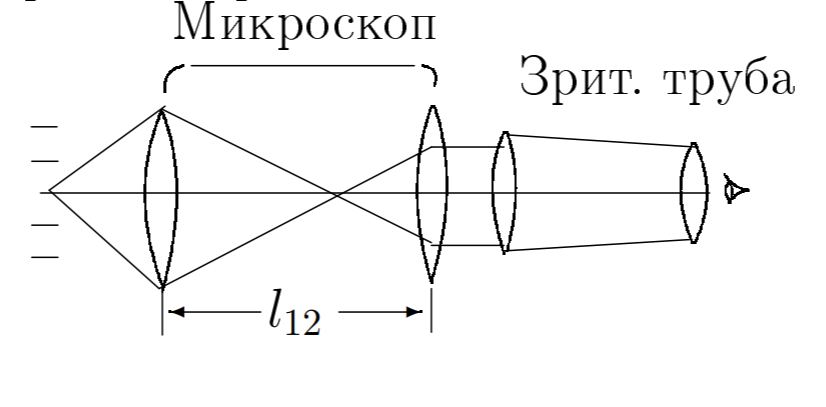
\includegraphics[width = 0.5\textwidth]{412-4.png}
				\caption{Модель микроскопа}
			\end{center}
		\end{figure}
		\item Расположили за окуляром модели микроскопа зрительную трубу, настроен-
		ную на бесконечность. Слегка перемещая осветитель, получили в поле зрения
		трубы изображение миллиметровой сетки. 
		
		\item Для экспериментального определения увеличения микроскопа измерили величину изображения $h_2$ миллиметрового деления предметной шкалы в делениях окулярной шкалы зрительной трубы:
		\begin{equation*}
		h_2 = 27\pm1\text{ дел./мм}.
		\end{equation*}
		Используя результат аналогичных измерений с коллиматорной линзой ($h_1$ в п. 2 модели телескопа Кеплера), фокус $f_3 = 19{,}5$ см которой известен, рассчитали увеличение микроскопа по формуле:
		\begin{equation*}
		N_m = -\dfrac{h_2}{h_1}\dfrac{L}{f_3} = 4{,}5\pm0{,}4.
		\end{equation*}
		Результат сравнили с теоретическим рассчётом увеличения микроскопа.
	\end{enumerate}

\subsection*{Выводы}
Определили фокусные расстояния собирающих и рассеивающих линз двумя способами, смоделировали ход лучей в трубе Галилея, трубе Кеплера и микроскопе, определили их увеличение разными способами и сравнили результаты. С точностью до погрешности результаты расчётов совпали, что подтверждает справедливость теоретических формул.

\end{document}
